\documentclass[12pt]{article}
\usepackage[margin=1.27cm]{geometry}
\usepackage{setspace}
\usepackage{fontspec}
% \usepackage[T1]{fontenc}
% \usepackage[utf8]{inputenc}
\usepackage{amsmath,txfonts,amssymb,nicefrac,mathtools,pifont} %for math
\usepackage{array,tabularx,multirow,fmtcount} %for tables
\usepackage{tikz, pgfplots} %for diagram
\usepackage{multicol} %for multiple column
\usepackage{enumerate,enumitem,adjustbox} %for ordered list
\usepackage{graphicx,subcaption,wrapfig,tcolorbox} %for figure
\usepackage{xparse} %for commands & environments
\usepackage{lipsum} %miscellaneous
\usepackage{colortbl,xcolor,soul} %for default table & border

% #ANCHOR Font settings
\setmainfont{Oxygen}
\newfontfamily\banglafont[Script=Bengali]{Baloo Da 2}
\newfontfamily{\lstsansserif}{IBM Plex Mono}
\renewcommand{\normalsize}{\fontsize{11.5pt}{13pt}\selectfont}


\setlength{\arrayrulewidth}{0.35 pt}
\definecolor{border}{HTML}{A1A1AA}
\arrayrulecolor{border}


% #ANCHOR Document settings
\linespread{1.45}
\setlength\parindent{0pt}
\setlength\parskip{16pt}
\setlist[enumerate]{noitemsep}
\usetikzlibrary{shapes.geometric,decorations.pathreplacing,trees,arrows,positioning,shapes,fit,calc,decorations.markings, decorations.text}
\tikzset{every node/.append style={font=\footnotesize}}
\usepgfplotslibrary{fillbetween}
\pgfdeclarelayer{background}
\pgfsetlayers{background,main}
\pgfplotsset{compat=1.18}
\columnseprule=1pt
\everymath{\displaystyle}
% #ANCHOR Hypernation
\tolerance=1
\emergencystretch=\maxdimen
\hyphenpenalty=10000
\hbadness=10000
\newlength{\colWidth}



% #ANCHOR Colors
\definecolor{azure(colorwheel)}{rgb}{0.0, 0.5, 1.0}
\definecolor{carminepink}{rgb}{0.92, 0.3, 0.26}
\definecolor{orange}{rgb}{0.9, 0.55, 0.22}
\definecolor{violet}{rgb}{0.60, 0.45, 1}
% Syantax Highlighting Colors
\definecolor{keyword}{HTML}{D73A4A}
\definecolor{number}{HTML}{015CC5}
\definecolor{comment}{HTML}{6A737D}
\definecolor{string}{HTML}{1D825E}
\definecolor{function}{HTML}{743FD1}
\definecolor{orange}{HTML}{CF7842}
\definecolor{codeblack}{HTML}{24292F}
\definecolor{divider}{HTML}{A1A1AA}
\definecolor{border}{HTML}{D1D1D1}


% #ANCHOR Ordered & Unordered List
\setlist[itemize,1]{left=0cm, label={\textbullet}}
\setlist[itemize,2,3,4,5,6,7,8,9,10]{left=0.6cm, label={\textbullet}}
\setlist[enumerate,1]{left=0cm}
\setlist[enumerate,2,3,4,5,6,7,8,9,10]{left=0.6cm}
\setul{0.5ex}{0.125ex}



% #ANCHOR Colored Box
\let\oldul\ul
\renewcommand{\ul}[2][keyword]{\text{\setulcolor{#1}\oldul{#2}}}
\newcommand{\redbox}[1]{%
{\color{red}\fbox{\color{black}#1}}
}
\newcommand{\red}[1]{%
\textcolor{red}{#1}
}
\newcommand{\redeq}[1]{%
\text{\color{red}$#1$}
}
\newcommand{\mred}[1]{%
\textcolor{keyword}{#1}
}
\newcommand{\mredeq}[1]{%
\textcolor{keyword}{$#1$}
}
\newcommand{\blue}[1]{%
% {\color{number}#1\hspace{-0.4ex}}
\textcolor{number}{#1}
}
\newcommand{\blueeq}[1]{%
\text{\color{number}$#1$}
}
\newcommand{\cyanbox}[1]{%
{\color{teal}\fbox{\textcolor{black}{#1}}}
}
\newcommand{\cyan}[1]{%
\textcolor{teal}{#1}
}
\newcommand{\pink}[1]{%
\textcolor{magenta}{#1}
}
\newcommand{\orange}[1]{%
\textcolor{orange}{#1}
}
\newcommand{\violet}[1]{%
{\color{violet}#1}
}
\newcommand{\cyaneq}[1]{%
\text{\color{teal}$#1$}
}
\newcommand{\gray}[1]{%
\textcolor{comment}{#1}
}
\newcommand{\pinkeq}[1]{%
\text{\color{magenta}$#1$}
}
\renewcommand{\columnseprulecolor}{\color{divider}}




% #ANCHOR Tabular commands
\newcolumntype{P}[1]{>{\centering\arraybackslash}p{#1}}
\newcolumntype{M}[1]{>{\centering\arraybackslash}m{#1}}
\newcolumntype{C}{>{\centering\arraybackslash}X}
\newcommand{\rspan}[2]{\multirow{#1}{*}{#2}}
\newcommand{\thc}[1]{%
\multicolumn{1}{|c|}{\textbf{#1}}
}
\newcommand{\thcx}[1]{%
\multicolumn{1}{|C|}{\textbf{#1}}
}
\newcommand{\thl}[1]{%
\multicolumn{1}{|l|}{\textbf{#1}}
}
\newcommand{\thr}[1]{%
\multicolumn{1}{|r|}{\textbf{#1}}
}
% Adjusting arraystretch to modify vertical padding
\renewcommand{\arraystretch}{1.25}
% Adjusting tabcolsep to modify horizontal padding
\setlength{\tabcolsep}{10pt}



% #ANCHOR Math commands
\newcommand{\set}[1]{\{$#1$\}}
\newcommand{\tabs}{\ \ \ \ \ \ }
\newcommand{\tab}{\ \ \ }
\newcommand{\cmark}{\ding{51}}%
\newcommand{\xmark}{\ding{55}}%
\newcommand{\boldi}[1]{\boldsymbol{#1}}%
\newcommand{\wspace}{\ \ = \ \ }



% #ANCHOR New commands
\newcommand{\Title}[1]{%
   \begin{center}
      \textbf{\Large{#1}}
   \end{center}
}
\newcommand{\Heading}[1]{%
   \par\vspace{\dimexpr -\baselineskip + 16pt}
   {\fontsize{12pt}{13pt}\selectfont\textbf{#1}}
   \par\vspace{\dimexpr -\baselineskip + 6pt}
}
\newcommand{\BuleHeading}[1]{%
   \par\vspace{\dimexpr -\baselineskip + 16pt}
   {\fontsize{12pt}{13pt}\selectfont\textbf{\textcolor{number}{#1}}}
   \par\vspace{\dimexpr -\baselineskip + 6pt}
}
\newcommand{\CHeading}[1]{%
   \par\vspace{\dimexpr -\baselineskip + 16pt}
   \hspace{\fill}
   {\fontsize{12pt}{13pt}\selectfont\textbf{#1}}
   \hspace{\fill}
   \par\vspace{\dimexpr -\baselineskip + 6pt}
}
\newcommand{\Section}[1]{%
   \par\vspace{\dimexpr -\baselineskip + 16pt}
   \hspace{\fill}
   {\fontsize{13pt}{13pt}\selectfont\textbf{#1}}
   \hspace{\fill}
   \par\vspace{\dimexpr -\baselineskip + 6pt}
}
\newcommand{\seteqno}[1]{%
   \ \cdots \ \cdots \ \cdots \ (#1)
}
\newcommand{\eqor}{%
   \Rightarrow \ \ 
}
\newcommand{\tsub}[1]{%
\textsubscript{#1}\hspace{-0.45ex}
}
\newcommand{\tsup}[1]{%
\textsuperscript{#1}\hspace{-0.45ex}
}
\newcommand{\cbox}[2][cyan]{
\tikz\node[draw=#1,circle,inner sep=2pt,baseline=(a.base)](a){#2};
}
\newcommand{\hrline}{%
\vspace{1ex} {\color{gray}\hrule} \vspace{4ex}
}
\newcommand{\divideX}[1][divider]{{\hspace{1ex}\color{#1}{\vrule}\hspace{1ex}}}
\newcommand{\Reference}[2][Reference]{

\vspace{-0.5\baselineskip}
\begin{center}
   {\fontspec{Merriweather}\textbf{#1:} \textit{#2}} 
\end{center}
}
\newcommand{\bn}[1]{%
   {\banglafont #1}
}

\NewDocumentCommand{\Column}{O{0.49} O{1.5em} m m}{
   \setlength{\colWidth}{\linewidth-#1\linewidth-#2}
   \begin{minipage}[t]{#1\linewidth}
      \noindent
         #3
      \end{minipage}\hspace{\fill}{\color{divider}\vrule width 0.35pt}\hspace{\fill}
      \begin{minipage}[t]{\colWidth}
      \noindent
         #4
   \end{minipage}
}

% New commands
\newcommand{\ro}[2][]{
\tab \xrightarrow[\scalebox{1}{$#1$}]{\scalebox{1}{$#2$}} \tab
}
\renewcommand{\vec}[1]{$\overrightarrow{#1}$}

\renewenvironment{pmatrix}
{\left(\begin{array}{ccc}}
{\end{array}\right)}

\NewDocumentEnvironment{fmatrix}{m}
{\left(\begin{array}{#1}}
{\end{array}\right)}

\NewDocumentEnvironment{pomatrix}{mm}
{\left(\begin{array}{ccc}}
{\end{array}\right)_{#1 \times #2}}

\NewDocumentEnvironment{figmatrix}{moO{0.3}}
{  
   \begin{subfigure}{#3\textwidth} \centering $$
      \begin{fmatrix}{#1}
}
{
      \end{fmatrix} $$ \IfValueT{#2}{#2}
   \end{subfigure}
}
\NewDocumentEnvironment{csplit}{o}
{  
   \IfValueT{#1}{\begin{center}}
      \begin{tabular}{l|l}
}
{
      \end{tabular}
   \IfValueT{#1}{\end{center}}
}
\newcommand{\sxrightarrow}[2][]{%
  \mathrel{\text{$\xrightarrow[#1]{#2}$}}%
}

   


\begin{document}
\Lecture{MTH 103: Linear Alzebra}

\Heading{Matrix}

\begin{equation*}
   A=\left[\begin{array}{ll}
   1 & 2 \\
   2 & 6
   \end{array}\right]_{2 \times 2} \quad B=\left[\begin{array}{ll}
   2 & 1 \\
   3 & 5
   \end{array}\right]_{2 \times 2}
\end{equation*}

\Topic{Addition and Subtraction:}
Two matrices can be added or subtracted if,

$\bullet$ The order of the matrices is equal. \tab or \tab $\bullet$ Their corresponding entries are equal.


\Topic{Multiplication:}
Two matrices can be multiplied if the number of the column in the first matrix is equal to the row in the second matrix.
\begin{equation*}
A = \begin{pomatrix}{2}{\red{3}}
      1 & 2 & 3 \\ 2 & 3 & 4
   \end{pomatrix}
   \quad B=
   \begin{pomatrix}{\red{3}}{2}
      1 & 1 \\ 2 & 0 \\ 3 & -1
   \end{pomatrix}
   \quad \therefore AB=
   \begin{pmatrix}
      1+4+9 & 1+0-3 \\ 2+6+12 & 2+0-4
   \end{pmatrix}
   \ = \ 
   \begin{pomatrix}{2}{2}
      19 & -2 \\ 20 & -2
   \end{pomatrix}
\end{equation*}


\Topic{Different types of matrices:}
\begin{figure}[h]
   \centering
   \begin{figmatrix}{ccc}[Zero matrix]
      0 & 0 & 0 \\ 0 & 0 & 0 \\ 0 & 0 & 0
   \end{figmatrix}
   \hfill
   \begin{figmatrix}{ccc}[Diagonal matrix]
      1 & 0 & 0 \\ 0 & 2 & 0 \\ 0 & 0 & 5
   \end{figmatrix}
   \hfill
   \begin{figmatrix}{ccc}[Identity matrix]
      1 & 0 & 0 \\ 0 & 1 & 0 \\ 0 & 0 & 1
   \end{figmatrix}
\end{figure}


\pagebreak
\vspace*{-\baselineskip}
\Heading{Determinant}

\begin{csplit}[c]
   $A= \begin{pmatrix}
      a_{11} & a_{12} \\ a_{21} & a_{22}
   \end{pmatrix} $
   \tabs & \tabs
   Determinant of $A$, \tab $|A| = (a_{11} a_{22}-a_{12} a_{21}) \tab \in R$
\end{csplit}


\Topic{Minors and Co-factor:}
\begin{csplit}[c]
   $\begin{pmatrix}
      3 & 1 & -4 \\ 2 & 5 & 6 \\ 1 & 4 & 8
   \end{pmatrix}$
   \tabs & \tabs
   $\therefore M_{32}=\left(\begin{array}{ll}
      3 & 4 \\ 2 & 6
   \end{array}\right)=26$
   \tabs \tabs
   $\therefore C_{32}= (-1)^{3+2} \ \cdot \
   \left(\begin{array}{ll}
      3 & 4 \\ 2 & 6
   \end{array}\right) = -26$
\end{csplit}


\Topic{Determinant Properties:}
\vspace*{1ex}
\begin{minipage}[t]{0.2\textwidth}
   \vspace*{-\baselineskip}
   \begin{equation*}
      |A| = \left|\begin{array}{cccc}
      a_{11} & \ldots & a_{1n} \\
      \vdots & & \vdots \\
      a_{n1} & \ldots & a_{nn}
      \end{array}\right|
   \end{equation*}
\end{minipage}
\hspace{1.25cm}
\begin{minipage}[t]{0.45\textwidth}
   $|A| = 0$; if one row/column is zero.\\
   $|A| = 0$; if two rows/columns are identical.
   $|AB| = |A| \cdot |B|$\\
   $|A+B| \neq |A|+|B|$
\end{minipage}
\hspace{0.6cm}
\begin{minipage}[t]{0.2\textwidth}
   $|A^{-1}| = \frac{1}{|A|}$ \\
   $|KA| = (K)^n\ |A|$ \\
   $|KA^{-1}| = K^n\ \frac{1}{|A|}$ \\
   $|(KA)^{-1}| = \frac{1}{K^n \cdot |A|}$
 \end{minipage}


\Topic{Inverse matrix}
\vspace*{2ex}
\begin{minipage}[t]{0.2\textwidth}
$A=\begin{pmatrix}
   a_{11} & a_{12} & a_{13} \\
   a_{21} & a_{22} & a_{23} \\
   a_{31} & a_{32} & a_{33}
\end{pmatrix}$
\end{minipage}
\hspace{1.25cm}
\begin{minipage}[t]{0.3\textwidth}
\vspace*{-\baselineskip}
   $|A|=a_{11} C_{11}+a_{12} C_{12}+a_{13} C_{13}$
   
   $A^{-1} \text{ exists if \ } |A| \neq 0$
   
\end{minipage}
\hspace{0.6cm}
\begin{minipage}[t]{0.3\textwidth}
\vspace*{-\baselineskip}
\cyanbox{Verification:}\\
If $A^{-1} = B$ \ then \ $AB=BA=I_n$\\
or, \ $A \cdot A^{-1}=I_n$
\end{minipage}


\vspace*{2ex}
\Topic{Inverse matrix of $(A)$ using Adjoint/Co-factor matrix}
\begin{equation*}
A = \begin{pmatrix}
      2 & 2 & 0 \\ 2 & 1 & 1 \\ -7 & 2 & -3
   \end{pmatrix}
\quad \begin{array}{ll} 
& |A| \ =\ 2(-3-2)+2(-7+6)+0=-12 \\
& \text { since }|A| \neq 0 \text {, then } A^{-1} \text { exists. }
\end{array}
\end{equation*}


Co-factors of the matrix,
$$\begin{array}{lll}
C_{11}=-5 \tabs & \tabs C_{21}=6 \tabs & \tabs C_{31}=2 \\
C_{12}=-1 \tabs & \tabs C_{22}=-6 \tabs & \tabs C_{32}=-2 \\
C_{13}=11 \tabs & \tabs C_{23}=-18 \tabs & \tabs C_{33}=-2 \\
\end{array}$$

\vspace{-0.5\baselineskip}
\begin{equation*}
   \therefore \operatorname{\ Adj }(A) \tab = \tab \left[C_{ij}\right]^T \tab = \tab \begin{pmatrix}
      -5 & 6 & 2 \\ -1 & -6 & -2 \\ 11 & -18 & -2
   \end{pmatrix}\\   
\end{equation*}

\begin{equation*}
\therefore A^{-1} \tab = \tab \frac{1}{|A|} \operatorname{\ AdJ }(A) \tab = \tab \frac{1}{-12}
\begin{pmatrix}
   -5 & 6 & 2 \\ -1 & -6 & -2 \\ 11 & -18 & -2
\end{pmatrix}
\end{equation*}

\Topic{Alternative way for determinant:}
\# Determinant of $(A)$ by co-factor expansion along first
row:\\
$|A| \tab = \tab a_{11} C_{11}+a_{12} C_{12}+a_{13} C_{13} \tab = \tab 2(-5)+2(-1)+0(11) \tab = \tab -12$

\# Determinant of $(A)$ by co-factor expansion along second
column:\\
$|A| \tab = \tab a_{12} C_{12}+a_{22} C_{22}+a_{32} C_{32} \tab = \tab 2(-1)+1(-6)+2(-2) \tab = \tab -12$

\# Determinant of $(A)$ by co-factor expansion along second
row:\\
$|A| \tab = \tab a_{21} C_{21}+a_{22} C_{22}+a_{23} C_{23} \tab = \tab 2(6)+1(-6)+1(-18) \tab = \tab -12$



\Heading{Solving system of linear equation : \cyan{Crammer's rule} }
If $AX=B$ is a system of $m$ linear equations in $n$ unknowns such that determinant \cyanbox{$D \neq 0$}, the system has a unique solution. This solution is,
$$x=\frac{Dx}{D}, \tabs y=\frac{Dy}{D}, \tabs z=\frac{Dz}{D}$$

\hrline

\cyanbox{Problem:} Solve the system of linear equations:
\begin{equation*}
\left.\begin{array}{rl}
2x+3 y & =60 \\
-6x+7 y & =40
\end{array}\right\} \tab \seteqno{1}
\end{equation*}

Write $(1)$ in matrix form $A \mathbf{x}=\mathbf{b}$,

\begin{equation*}
   \begin{aligned}
   & A= \begin{fmatrix}{cc}
      2 & 3 \\ -6 & 7
   \end{fmatrix} \tabs \mathbf{x}= \begin{fmatrix}{l}
      x \\ y
   \end{fmatrix}\tabs \mathbf{b}=\begin{fmatrix}{l}
      60 \\ 40
   \end{fmatrix}\\&\\
   & \therefore D=\begin{fmatrix}{cc}
   2 & 3 \\ -6 & 7
   \end{fmatrix} \tab = 14+18=32 \\
   & \therefore Dx=\begin{fmatrix}{ll}
   60 & 3 \\ 40 & 7
   \end{fmatrix} \tab = 420-120 = 300 \tabs \therefore x=\frac{D x}{D}=\frac{300}{32}=\frac{75}{8} \\ & \therefore Dy=\begin{fmatrix}{cc}
   2 & 60 \\ -6 & 40
   \end{fmatrix} \tab = 80+360 = 440 \tabs \therefore y=\frac{D y}{D}=\frac{440}{32}=\frac{55}{4} \\
   &  \\ & \therefore\begin{fmatrix}{l}
   x \\ y
   \end{fmatrix}=\begin{fmatrix}{l}
      \scalebox{1.5}{\nicefrac{$75$}{$8$}} \\ \scalebox{1.5}{\nicefrac{$55$}{$4$}}
   \end{fmatrix} \\
   &
   \end{aligned}
\end{equation*}

\vspace{5ex}
\cyanbox{Problem:} Solve the system of linear equations,
\begin{equation*}
   \left.\begin{array}{rl}
      x_1-2 x_2+3 x_3=7 \\ 2 x_1+x_2-x_3=1 \\ x_1-x_2-x_3=-6
   \end{array}\right\} \tab \seteqno{1}
\end{equation*}

Write $(1)$ in matrix form, $A \mathbf{x}=\mathbf{b}$
\begin{equation*}
   A=\begin{fmatrix}{ccc}
         1 & -2 & 3 \\ 2 & 1 & -1 \\ 1 & -1 & -1
      \end{fmatrix} \tabs \mathbf{x}=\begin{fmatrix}{l}
      x_1 \\ x_2 \\ x_3
      \end{fmatrix} \tabs \mathbf{b}=\begin{fmatrix}{c}
         7 \\ 1 \\ -6
      \end{fmatrix}
\end{equation*}
$$\therefore D=|A| \ = \ 1(-1-1)+2(-2+1)+3(-2-1)\ = \ -13$$

Since $D \neq 0$, the system has a unique solution.

\begin{equation*}
   \begin{aligned}
   & \therefore Dx_1=\begin{fmatrix}{ccc}
      7 & -2 & 3 \\ 1 & 1 & -1 \\ -6 & -1 & -1
   \end{fmatrix}=-13 \tabs \therefore x_1 = \frac{Dx_1}{D} = \frac{-13}{-13}=1\\
   & \therefore Dx_2=\begin{fmatrix}{ccc}
      1 & 7 & 3 \\ 2 & 1 & -1 \\ 1 & -6 & -1
   \end{fmatrix}=-39 \tabs \therefore x_2 = \frac{Dx_2}{D} = \frac{-39}{-13}=3\\
   & \therefore Dx_3=\begin{fmatrix}{ccc}
      1 & -2 & 7 \\ 2 & 1 & 1 \\ 1 & -1 & -6
   \end{fmatrix}=-52 \tabs \therefore x_3 = \frac{Dx_3}{D} = \frac{-52}{-13}=4
\end{aligned}
\end{equation*}

\begin{equation*}
   \begin{aligned}
   & \therefore\begin{fmatrix}{l}
   x_1 \\ x_2 \\ x_3
   \end{fmatrix}=\begin{fmatrix}{l}
      1 \\ 3 \\ 4
   \end{fmatrix}
   \end{aligned}
\end{equation*}


\Heading{Elementary Matrices for Fing $A^{-1}$}
\Topic{Elementary row operation (e.r.o):}
\tabs (1) Multiply a row by a non-zero constant $C$

\tabs (2) Interchange two rows

\tabs (3) Add $C$ times one row to another.

\Topic{Row equivalent matrix:}
Matrices $A$ and $B$ are said to be row equivalent if each of them can be obtained from the other by a sequence of elementary row operations (e.r.o.)

\begin{equation*}
A= \begin{pmatrix}
   1 & 1 & 2 \\ 0 & 1 & 5 \\ 2 & 3 & 4
\end{pmatrix} 
\ro{R_2 \leftrightarrow R_3}
\begin{pmatrix}
   1 & 1 & 2 \\ 2 & 3 & 4 \\ 0 & 1 & 5
\end{pmatrix}
\ro{R_3' = -2R_3}
\begin{pmatrix}
   1 & 1 & 2 \\ 2 & 3 & 4 \\ 0 & -2 & -10
\end{pmatrix} =B
\end{equation*}
\begin{equation*}
B= \begin{pmatrix}
   1 & 1 & 2 \\ 2 & 3 & 4 \\ 0 & -2 & -10
\end{pmatrix} 
\ro{R_3' = -\frac{1}{2}R_3}
\begin{pmatrix}
   1 & 1 & 2 \\ 2 & 3 & 4 \\ 0 & 1 & 5
\end{pmatrix}
\ro{R_2 \leftrightarrow R_3}
\begin{pmatrix}
   1 & 1 & 2 \\ 0 & 1 & 5 \\ 2 & 3 & 4
\end{pmatrix} =A
\end{equation*}

\Topic{Elementary matrix:}
A matrix $E$ is called an elementary matrix if it can be obtained from an identity matrix by performing a single elementary row operation. $I \stackrel{\text{ \ e.r.o \ }}{\longrightarrow} E$.


\vspace{3ex}
\cyanbox{\# Problem} Find an elementary matrix $E$ that satisfies $EB=D$

\begin{equation*}
   B =\begin{pmatrix}
      8 & 1 & 5 \\ 2 & -7 & -1 \\ 3 & 4 & 1
   \end{pmatrix} \quad \quad D=\begin{pmatrix}
      8 & 1 & 5 \\ -6 & 21 & 3 \\ 3 & 4 & 1
   \end{pmatrix} \\
\end{equation*}
\begin{equation*}
   I_3 =\begin{pmatrix}
      1 & 0 & 0 \\ 0 & 1 & 0 \\ 0 & 0 & 1
   \end{pmatrix} \ro{R_2'=-3R_2}\begin{pmatrix}
      1 & 0 & 0 \\ 0 & -3 & 0 \\ 0 & 0 & 1
   \end{pmatrix}=E \\
\end{equation*}
   \begin{equation*}
   \therefore EB =\begin{pmatrix}
      1 & 0 & 0 \\ 0 & -3 & 0 \\ 0 & 0 & 1
   \end{pmatrix}\begin{pmatrix}
      8 & 1 & 5 \\ 2 & -7 & -1 \\ 3 & 4 & 1
   \end{pmatrix}=\begin{pmatrix}
      8 & 1 & 5 \\ -6 & 21 & 3 \\ 3 & 9 & 1
   \end{pmatrix}_\text { (proved) }
\end{equation*}

\Heading{Row Echelon form (REF) / \cyan{Gaussian Elimination}}
A matrix is in echelon form if -
\begin{enumerate}[label=(\arabic*)]
   \item Non-zero rows appear above the zero rows.
   \item In any non-zero row, the first non-zero element (called the leading element) appears to the left of the leading element in any lower row.
\end{enumerate}

\pagebreak
\cyanbox{Problem:} Determine whether the matrix is in Row Echelon Form or not.

\begin{figure}[h]
   \centering
   \begin{figmatrix}{lll}[\checkmark][0.17]
      1 & 0 & 0 \\ 0 & 1 & 0 \\ 0 & 0 & 1
   \end{figmatrix}
   \begin{figmatrix}{lll}[\checkmark][0.17]
      1 & 0 & 0 \\ 0 & 1 & 0 \\ 0 & 0 & 0
   \end{figmatrix} 
   \begin{figmatrix}{lll}[$\times$][0.17]
      1 & 0 & 0 \\ 0 & 0 & 1 \\ 0 & \pinkeq{1} & 0
   \end{figmatrix}
   \begin{figmatrix}{lll}[\checkmark][0.17]
      1 & 2 & 3 \\ 0 & 1 & 4 \\ 0 & 0 & 9
   \end{figmatrix}
   \begin{figmatrix}{lll}[\checkmark][0.17]
      1 & 2 & 3 \\ 0 & 2 & 3 \\ 0 & 0 & 1
   \end{figmatrix}
   \begin{figmatrix}{lll}[$\times$][0.17]
      1 & 2 & 3 \\ 0 & 1 & 2 \\ 0 & \pinkeq{1} & 5
   \end{figmatrix}
   \begin{figmatrix}{lll}[$\times$][0.17]
      1 & 2 & 3 \\ \pinkeq{0} & \pinkeq{0} & \pinkeq{0} \\ 0 & 1 & 5
   \end{figmatrix}
   \begin{figmatrix}{lllll}[\checkmark][0.17]
      1 & 2 & 3 & 4 & 5 \\
      0 & 1 & 2 & 3 & 4 \\
      0 & 0 & 0 & 1 & 2
   \end{figmatrix}
\end{figure}



\Heading{Reduced Row Echelon Form (RREF) / \cyan{Gauss-Jordan Elimination}}
If a column contains a leading element, all the other elements in that column are zero.

\begin{figure}[h]
   \centering
   \begin{figmatrix}{ccc}[$\times$][0.2]
      1 & \pinkeq{2} & \pinkeq{3} \\
      0 & 1 & \pinkeq{2} \\
      0 & 0 & 1
   \end{figmatrix}
   \begin{figmatrix}{ccc}[\checkmark][0.2]
      1 & 0 & 0 \\
      0 & 4 & 0 \\
      0 & 0 & 7
   \end{figmatrix}
   \begin{figmatrix}{ccccc}[$\times$][0.2]
      1 & \pinkeq{2} & 3 & 4 & 3 \\
      0 & 1 & 1 & 2 & 0 \\
      0 & 0 & 0 & 0 & 0
   \end{figmatrix}
   \begin{figmatrix}{ccccc}[\checkmark][0.2]
      1 & 0 & 3 & 4 & 5 \\
      0 & 1 & 1 & 2 & 0 \\
      0 & 0 & 0 & 0 & 0
   \end{figmatrix}
\end{figure}


\Topic{Augmented matrix}
An augmented matrix is a matrix obtained by appending the columns of two given matrices, usually to perform the same elementary row operation (e.r.o) on each of the given matrices.
\begin{equation*}
A=\begin{fmatrix}{lll}
   1 & 3 & 2 \\ 2 & 0 & 1 \\ 5 & 2 & 2
\end{fmatrix} \quad B=\begin{fmatrix}{l}
   4 \\ 3 \\ 1
\end{fmatrix} \quad
\therefore(A \mid B)=\begin{fmatrix}{lll|l}
   1 & 3 & 2 & 4 \\ 2 & 0 & 1 & 3 \\ 5 & 2 & 2 & 1
\end{fmatrix}
\end{equation*}

\vspace{2ex}
\cyanbox{\# Problem} Find the inverse of the given matrix.
\begin{equation*}
A=\begin{fmatrix}{lll}
   1 & 2 & 3 \\ 2 & 5 & 3 \\ 1 & 0 & 8
\end{fmatrix}
\end{equation*}

reduce it to reduce row echelon form by e.r.o
\begin{equation*}
\begin{aligned}
\therefore \left(A \mid I_3\right) =
& \begin{fmatrix}{lll|lll}
   1 & 2 & 3 & 1 & 0 & 0 \\
   2 & 5 & 3 & 0 & 1 & 0 \\
   1 & 0 & 8 & 0 & 0 & 1
\end{fmatrix}
   \ro[R_3'=R_3-R_1]{R_2'=R_2-2R_1}
\begin{fmatrix}{ccc|ccc}
   1 & 2 & 3 & 1 & 0 & 0 \\
   0 & 1 & -3 & -2 & 1 & 0 \\
   0 & -2 & 5 & -1 & 0 & 1
\end{fmatrix} \\ & \\
   \ro{R_3'=R_3+2R_2}
&\begin{fmatrix}{ccc|ccc}
   1 & 2 & 3 & 1 & 0 & 0 \\
   0 & 1 & -3 & -2 & 1 & 0 \\
   0 & 0 & -1 & -5 & 2 & 1
\end{fmatrix}
   \ro{R_3'=-R_3}
\begin{fmatrix}{ccc|ccc}
   1 & 2 & 3 & 1 & 0 & 0 \\
   0 & 1 & -3 & -2 & 1 & 0 \\
   0 & 0 & 1 & 5 & -2 & -1
\end{fmatrix} \\ & \\
   \ro[R_1'=R_1-3R_3]{R_2'=R_2+3R_3}
& \begin{fmatrix}{ccc|ccc}
   1 & 2 & 0 & -14 & 6 & 3 \\
   0 & 1 & 0 & 13 & -5 & -3 \\
   0 & 0 & 1 & 5 & -2 & -1
\end{fmatrix}
   \ro{R_1'=R_1-2R_2}
\begin{fmatrix}{ccc|ccc}
   1 & 0 & 0 & -40 & 16 & 9 \\
   0 & 1 & 0 & 13 & -5 & -3 \\
   0 & 0 & 1 & 5 & -2 & -1
\end{fmatrix} \\ & \\
   & \therefore A^{-1}=
\begin{fmatrix}{ccc}
   -40 & 16 & 9 \\
   13 & -5 & -3 \\
   5 & -2 & -1
\end{fmatrix}
\end{aligned}
\end{equation*}



\pagebreak
\vspace*{-\baselineskip}
\Heading{System of linear equation}
\begin{equation*}
\begin{matrix}
   ax+by+c & \tabs \tabs & x^2+y^2=1\\
   \text{linear equation} && \text{polynomial equation} \\[2ex]
   & \cyanbox{variables $\rightarrow$ unknowns} &
\end{matrix}
\end{equation*}

{\large
\begin{equation*}
   \begin{matrix}
      a_{\cyaneq{1}1}x_{\redeq{1}} &+& a_{12}x_{\redeq{2}} &+& \cdots &+& a_{1n}x_{\redeq{n}} &=& b_1\\
      a_{\cyaneq{2}1}x_{\redeq{1}} &+& a_{22}x_{\redeq{2}} &+& \cdots &+& a_{2n}x_{\redeq{n}} &=& b_2\\
      \vdots &&&&&& \vdots && \vdots\\
      a_{\cyaneq{m}1}x_{\redeq{1}} &+& a_{m2}x_{\redeq{2}} &+& \cdots &+& a_{mn}x_{\redeq{n}} &=& b_n
   \end{matrix}
\end{equation*}
}


It can be expressed in matrix form $A \mathbf{x}=\mathbf{b}$,
\begin{equation*}
A = [a_{ij}]=\begin{fmatrix}{llll}
a_{11} & a_{12} & \ldots & a_{1n} \\
a_{21} & a_{22} & \ldots & a_{2n} \\
\vdots & \vdots && \vdots \\
a_{m1} & a_{m2} & \ldots & a_{mn}
\end{fmatrix}, \quad
\mathbf{x} = [x_{i}] = \begin{fmatrix}{l}
x_1 \\ x_2 \\ \vdots \\ x_n
\end{fmatrix}, \quad
\mathbf{b} = [b_{i}] = \begin{fmatrix}{c}
b_1 \\ b_2 \\ \vdots \\ b_n
\end{fmatrix}
\end{equation*}

% \vspace{2ex}
\begin{center}
   $a_{ij} \in R; \tabs b_i \in R$\\
   \cyaneq{m} equations \tab \& \tab \redeq{n} unknowns
\end{center}



\begin{multicols}{3}\centering   
   $\begin{aligned}
       x-y&=1\\[-1ex] 2x+y&=6 \\[2ex] 2x-2y&=2\\[-1ex] 2x+y&=6 \\[-3ex]\cline{1-2}\\[-6ex]-3y&=-4
   \end{aligned}$
   \vspace{-1ex}
   $$\therefore x=\scalebox{1.2}{\nicefrac{$7$}{$3$}} \tabs y=\scalebox{1.2}{\nicefrac{$4$}{$3$}}$$
   
   \vspace{-2ex}
  \fbox{equations $(\cyaneq{m})$ $=$ unknowns $(\redeq{n})$}\\[2ex]
   One $\backslash$ Unique solution

   \columnbreak

   $\begin{aligned}
      x+y&=4\\[-1ex] 3x+3y&=6 \\[2ex] 3x+3y&=12\\[-1ex] 3x+3y&=6\\[-3ex]\cline{1-2}\\[-6ex]0&=\pinkeq{6}
   \end{aligned}$
   $$\therefore 0=\pinkeq{b} \text{ \ and \ } \pinkeq{b} \neq 0$$
   
   \vspace{-2ex}
   \fbox{equations $(\cyaneq{m})$ $>$ unknowns $(\redeq{n})$}\\[2ex]
   No solution
   
   \columnbreak
   
   $\begin{aligned}
      4x-2y&=1\\[-1ex] 16x-8y&=4 \\[2ex] 4x-2y&=1\\[-1ex] 4x-2y&=1\\[-3ex]\cline{1-2}\\[-6ex]0&=\pinkeq{0}
   \end{aligned}$
   $$\therefore 0=\pinkeq{b} \text{ \ and \ } \pinkeq{b}=0$$

   \vspace{-2ex}
   \fbox{equations $(\cyaneq{m})$ $<$ unknowns $(\redeq{n})$}\\[2ex]
   Infinitely many solutions

   \fbox{Free variables: $n-m$}
\end{multicols}

\Heading{Types of solution for the system of linear equation}
\begin{center}
\begin{tikzpicture}
   [level 1/.style={sibling distance=10cm},
   level 2/.style={sibling distance=5cm}]

   \node{Consistent system}[edge from parent fork down]
   child {
      node {Non-homogeneous}
      node[below=5pt] {$(C \neq 0)$}
      child {
         node{Unique solution}
         node[below=10pt] {\centering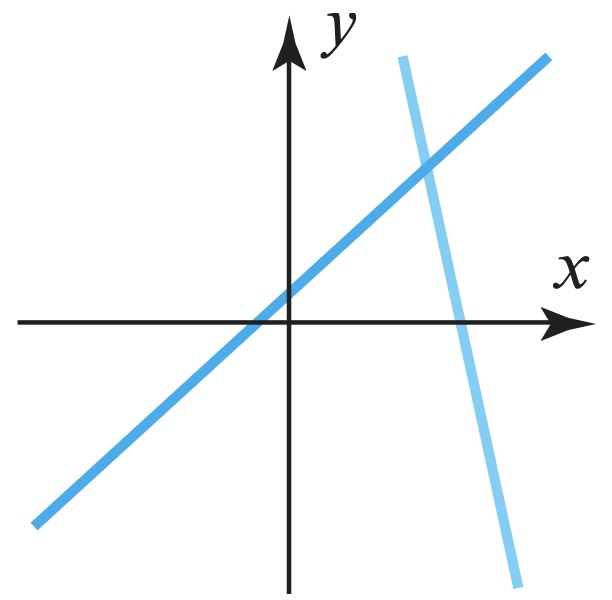
\includegraphics[width=25mm]{figures/Unique.JPG}}
         }
      child {
         node{Infinitely many solutions}
         node[below=10pt] {\centering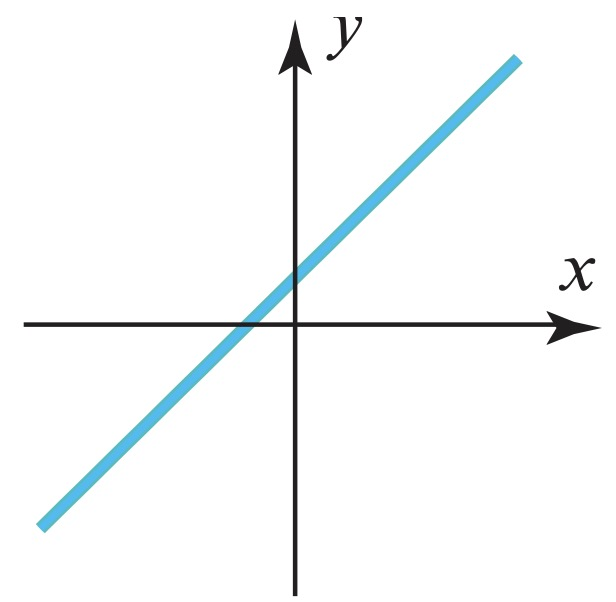
\includegraphics[width=25mm]{figures/InfinitelyMany.JPG}}
         }
   }
   child {
      node {Homogeneous}
      node[below=5pt] {$(C = 0)$}
      child {
         node{Trivial solution}
         node[below=10pt] {\centering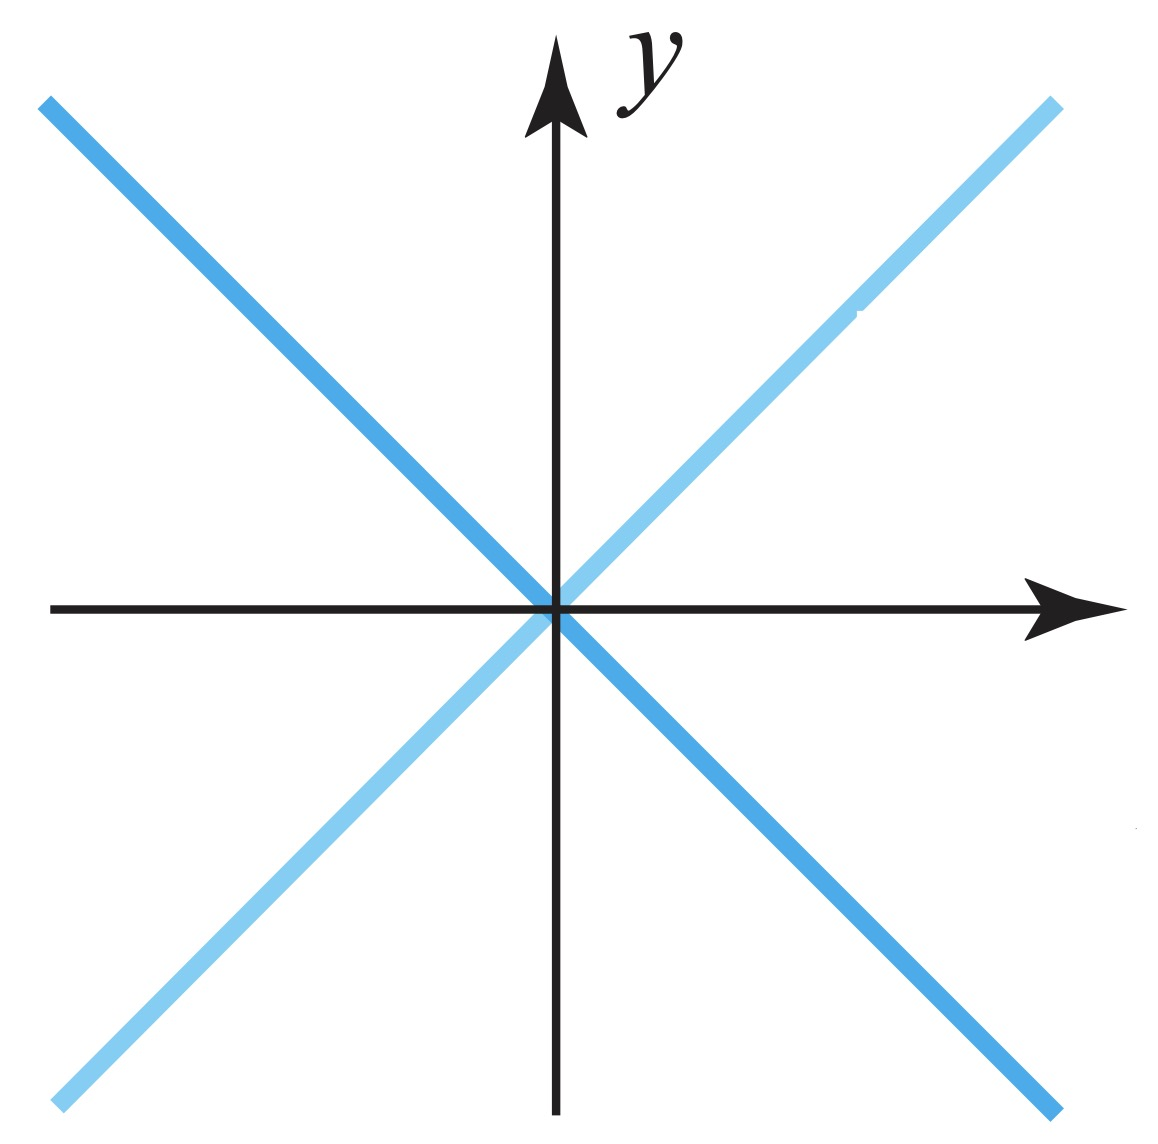
\includegraphics[width=25mm]{figures/Trivial.JPG}}
         }
      child {
         node{Non-trivial solution}
         node[below=10pt] {\centering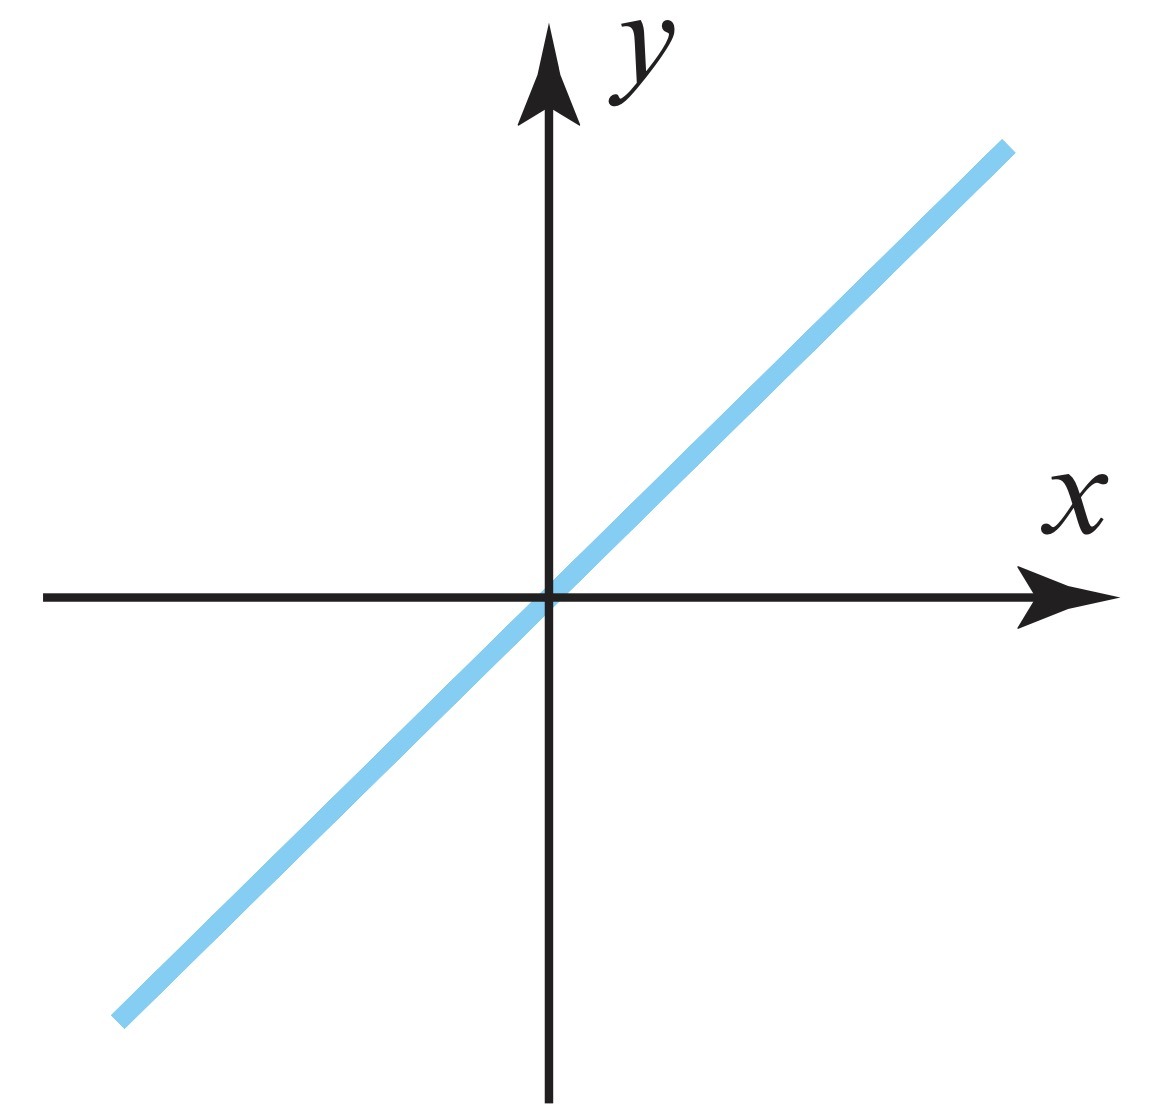
\includegraphics[width=25mm]{figures/NonTrivial.JPG}}
         }
   };
\end{tikzpicture}
\end{center}


\Heading{System of linear equations: \cyan{Exercises}}
\cyanbox{Problem:} Solve the system of linear equations
\begin{alignat*}{6}
   x &\ +\ & y &\ +\ & 2z &\ =\ & 9 \\
   2x &\ +\ & 4y &\ -\ & 3z &\ =\ & 1 \\
   3x &\ +\ & 6y &\ -\ & 5z &\ =\ & 0 \\
\end{alignat*}

\cyanbox{Solution:} Let,
\begin{equation*}
   \left.
   \begin{alignedat}{6}
      x &\ +\ & y &\ +\ & 2z &\ =\ & 9 \\
      2x &\ +\ & 4y &\ -\ & 3z &\ =\ & 1 \\
      3x &\ +\ & 6y &\ -\ & 5z &\ =\ & 0
   \end{alignedat}
   \tab \right\} \tab \seteqno{1}
\end{equation*}

In matrix form $A \mathbf{x}=\mathbf{b}$,
\begin{equation*}
   A=\begin{fmatrix}{rrr}
   1 & 1 & 2 \\ 2 & 4 & -3 \\ 3 & 6 & -5
   \end{fmatrix}, \quad
   \mathbf{x} \ = \ \begin{fmatrix}{l}
   x \\ y \\ z
   \end{fmatrix}, \quad
   \mathbf{b} \ = \ \begin{fmatrix}{r}
   9 \\ 1 \\ 0
   \end{fmatrix}
\end{equation*}

Reduce augmented matrix \ $(A \mid \mathbf{b})$ \ to row echelon form by e.r.o
\begin{equation*}
   \left(A \mid \mathbf{b}\right) = \ 
   \begin{fmatrix}{rrr|r}
      1 & 1 & 2 & 9 \\
      2 & 4 & -3 & 1 \\
      3 & 6 & -5 & 0
   \end{fmatrix}
      \ro[R_3'=R_3-3R_1]{R_2'=R_2-2R_1}
   \begin{fmatrix}{rrr|r}
      1 & 1 & 2 & 9 \\
      0 & 2 & -7 & -17 \\
      0 & 3 & -11 & -27
   \end{fmatrix}
      \ro{R_3'=2R_3+3R_2}
   \begin{fmatrix}{rrr|r}
      1 & 1 & 2 & 9 \\
      0 & 2 & -7 & -17 \\
      0 & 0 & -1 & -3
   \end{fmatrix}
\end{equation*}

This is in row echelon form.

Corresponding linear equations,
\vspace{-0.75\baselineskip}
\begin{align*}
   x+y+2z&=9\\
   2y-7z&=-17\\
   -z&=-3
\end{align*}

There is no equations in the form $0=b$ with $b \neq 0$

So the system is consistent and the system has a solution.

Since there are $3$ unknowns is $3$ equations, so the system has a unique solution.


\vspace{2ex}
By backward substition,
\begin{equation*}
\begin{aligned}
& z=3 \\ & y=2 \\ & x=1
\end{aligned} \tabs \tabs \tabs \tabs \therefore \mathbf{x}=\left(\begin{array}{l}
x \\ y \\ z
\end{array}\right)=\left(\begin{array}{l}
1 \\ 2 \\ 3
\end{array}\right) \text { is the solution. }
\end{equation*}



\vspace{5ex}
\hrline
\cyanbox{Problem:} Solve the system of linear equations
\begin{alignat*}{12}
   x_1 &\ -\ & 3x_2 &\ -\ & 2x_3 &&&\ +\ & 2x_5 &&&\ =\ & 0 \\
   2x_1 &\ +\ & 6x_2 &\ -\ & 5x_3 &\ -\ & 2x_4 &\ +\ & 4x_5 &\ -\ & 3x_6 &\ =\ & -1 \\
   &&&&5x_3 &\ +\ & 10x_4 &&&\ +\ & 15x_6 &\ =\ & 5 \\
   2x_1 &\ +\ & 6x_2 &&&\ +\ & 8x_4 &\ +\ & 4x_5 &\ +\ & 18x_6 &\ =\ & 6 \\
\end{alignat*}

\cyanbox{Solution:} Let,
\begin{equation*}
   \left.
   \begin{alignedat}{1}
      x_1-3x_2-2x_3+2x_5 &=0 \\
      2x_1+6x_2-5x_3-2x_4+4x_5-3x_6 &=-1 \\
      5x_3+10x_4+15x_6 &=5 \\
      2x_1+6x_2+8x_4+4x_5+18x_6 &=6 \\
   \end{alignedat}
   \tab \right\} \tab \seteqno{1}
\end{equation*}

In matrix form $A \mathbf{x}=\mathbf{b}$,
\begin{equation*}
   A=\begin{fmatrix}{cccccc}
      1 & 3 & -2 & 0 & 2 & 0 \\
      2 & 6 & -5 & -2 & 4 & -3 \\
      0 & 0 & 5 & 10 & 0 & 15 \\
      2 & 6 & 0 & 8 & 4 & 18
   \end{fmatrix}, \quad
   \mathbf{x} \ = \ \begin{fmatrix}{l}
      x_1 \\ x_2 \\ x_3 \\ x_4 \\ x_5 \\ x_6
   \end{fmatrix}, \quad
   \mathbf{b} \ = \ \begin{fmatrix}{r}
      0 \\ -1 \\ 5 \\ 6
   \end{fmatrix}
\end{equation*}


Reduce augmented matrix \ $(A \mid \mathbf{b})$ \ to reduced row echelon form by e.r.o
\begin{align*}
   \left(A \mid \mathbf{b}\right) = \ 
   &\begin{fmatrix}{cccccc|c}
      1 & 3 & -2 & 0 & 2 & 0 & 0 \\
      2 & 6 & -5 & -2 & 4 & -3 & -1 \\
      0 & 0 & 5 & 10 & 0 & 15 & 5 \\
      2 & 6 & 0 & 8 & 4 & 18 & 6
   \end{fmatrix}
      \ro[R_4'=R_4-2R_1]{R_2'=R_2-2R_1}
   \begin{fmatrix}{cccccc|c}
      1 & 3 & -2 & 0 & 2 & 0 & 0 \\
      0 & 0 & -1 & -2 & 0 & -3 & -1 \\
      0 & 0 & 5 & 10 & 0 & 15 & 5 \\
      0 & 0 & 4 & 8 & 0 & 18 & 6
   \end{fmatrix}\\&\\
      \ro[R4'=R4+4R2]{R_3'=\frac{R3}{5}}
   &\begin{fmatrix}{cccccc|c}
      1 & 3 & -2 & 0 & 2 & 0 & 0 \\
      0 & 0 & -1 & -2 & 0 & -3 & -1 \\
      0 & 0 & 1 & 2 & 0 & 3 & 1 \\
      0 & 0 & 0 & 0 & 0 & 6 & 2
   \end{fmatrix}
      \ro{R_3'=R3+R2}
   \begin{fmatrix}{cccccc|c}
      1 & 3 & -2 & 0 & 2 & 0 & 0 \\
      0 & 0 & -1 & -2 & 0 & -3 & -1 \\
      0 & 0 & 0 & 0 & 0 & 0 & 0 \\
      0 & 0 & 0 & 0 & 0 & 6 & 2
   \end{fmatrix}\\&\\
      \ro[R3 \leftrightarrow R4]{R3'=-\ R3}
   &\begin{fmatrix}{cccccc|c}
      1 & 3 & -2 & 0 & 2 & 0 & 0 \\
      0 & 0 & 1 & 2 & 0 & 3 & 1 \\
      0 & 0 & 0 & 0 & 0 & 6 & 2 \\
      0 & 0 & 0 & 0 & 0 & 0 & 0
   \end{fmatrix}
      \ro[R1'=R1+R2]{R2'=2R2-R1}
   \begin{fmatrix}{cccccc|c}
      1 & 3 & 0 & 4 & 2 & 0 & 0 \\
      0 & 0 & 2 & 4 & 0 & 0 & 0 \\
      0 & 0 & 0 & 0 & 0 & 6 & 2 \\
      0 & 0 & 0 & 0 & 0 & 0 & 0
   \end{fmatrix}
\end{align*}

This is in reduced row echelon form.

Corresponding linear equations,
\vspace{-0.75\baselineskip}
\begin{align*}
   x_1+3x_2+4x_4+2x_5&=0\\
   2x_3+4x_4&=0\\
   6x_6&=2
\end{align*}

There is no equations in the form $0=b$ with $b \neq 0$

So the system is consistent and the system has a solution.

Since there are $6$ unknowns is $3$ equations, so the system has infinitely many solutions\\ and have $(6-3)=3$ free variables, namely $x_2$, $x_4$, $x_5$.


\vspace{2ex}
Let, \tab $x_2=r$, \tab $x_4=s$, \tab $x_5=t$


\vspace{2ex}
By backward substition, \tab 
$x_6=\frac{1}{3} \tabs \tab x_3=-2s \tabs \tab x_1=-3r-4s-2t$

\vspace{2ex}
The solution is,
\begin{align*}
\mathbf{x}&=\left(\begin{array}{c}
   x_1 \\ x_2 \\ x_3 \\ x_4 \\ x_5 \\ x_6
\end{array}\right)=\left(\begin{array}{c}
   -3r-4s-2t \\ r \\ -2s \\ s \\ t \\ \frac{1}{3}
\end{array}\right) \\&\\
&=\left(\begin{array}{c}
   0 \\ 0 \\ 0 \\ 0 \\ 0 \\ \frac{1}{3}
\end{array}\right)
+r\ \left(\begin{array}{c}
   -3 \\ 1 \\ 0 \\ 0 \\ 0 \\ 0
\end{array}\right)
+s\ \left(\begin{array}{c}
   -4 \\ 0 \\ -2 \\ 1 \\ 0 \\ 0
\end{array}\right)
+t\ \left(\begin{array}{c}
   -2 \\ 0 \\ 0 \\ 0 \\ 1 \\ 0
\end{array}\right)
\end{align*}


\vspace{10ex}
\cyanbox{Problem:} determine the values of $a$ for which the system has no solutions, exactly one solution, or infinitely many solutions.
\begin{alignat*}{6}
   x &\ +\ & 2y &\ -\ & 3z &\ =\ & 4 \\
   3x &\ -\ & y &\ +\ & 5z &\ =\ & 2 \\
   4x &\ +\ & y &\ +\ & (a^2-14)z &\ =\ & a+2
\end{alignat*}

In matrix form $A \mathbf{x}=\mathbf{b}$,
\begin{equation*}
   A=\begin{fmatrix}{ccc}
   1 & 2 & -3 \\ 3 & -1 & 5 \\ 4 & 1 & a^2-14
   \end{fmatrix}, \quad
   \mathbf{x} \ = \ \begin{fmatrix}{l}
   x \\ y \\ z
   \end{fmatrix}, \quad
   \mathbf{b} \ = \ \begin{fmatrix}{c}
   4 \\ 2 \\ a+2
   \end{fmatrix}
\end{equation*}


Reduce augmented matrix \ $(A \mid \mathbf{b})$ \ to row echelon form by e.r.o
\begin{align*}
   \left(A \mid \mathbf{b}\right) = \ 
   &\begin{fmatrix}{ccc|c}
      1 & 2 & -3 & 4 \\
      3 & -1 & 5 & 2 \\
      4 & 1 & a^2-14 & a+2
   \end{fmatrix}
      \ro[R_3'=R_3-4R_1]{R_2'=R_2-3R_1}
   \begin{fmatrix}{ccc|c}
      1 & 2 & -3 & 4 \\
      0 & -7 & 14 & -10 \\
      0 & -7 & a^2-2 & a-14
   \end{fmatrix}\\&\\
      \ro{R_3'=R3-R2}
   &\begin{fmatrix}{ccc|c}
      1 & 2 & -3 & 4 \\
      0 & -7 & 14 & -10 \\
      0 & 0 & a^2-16 & a-4
   \end{fmatrix}
\end{align*}

This is in row echelon form.

Corresponding linear equations,
\vspace{-0.75\baselineskip}
\begin{align*}
   x+2y-3z &=4 \\
   -7y+14z &=-10 \\
   (a-4)(a+4)z &=a-4
\end{align*}


Conclusion:

\begin{tabular}{lll}
   $a=-4$ &:& There is an equation of the form \ $0=b$ \ with \ $b \neq 0$ \\ &&So, the system is inconsistent and has no solution.\\[2ex]

   $a \neq \pm 4$ &:& There are 3 unknowns in 3 equations. \\ &&So, the system has exactly one solution.\\[2ex]

   $a=4$ &:& There are 3 unknowns in 2 equations. \\ &&So, the system has infinitely many solutions.
\end{tabular}



\pagebreak
\vspace*{-\baselineskip}
\Heading{Solving system of linear equation : \cyan{Inverting the coefficient matrix / using $A^{-1}$}}
\Reference{Exercise Set-1.6 (1-8) \ | \ Chapter-1 \ | \ Page-66}

\cyanbox{Problem:} Solve the system of linear equations using $A^{-1}$
\begin{alignat*}{6}
   x_1 &\ +\ & 2x_2 &\ +\ & 3x_3 &\ =\ & 5 \\
   2x_1 &\ +\ & 5x_2 &\ +\ & 3x_3 &\ =\ & 3 \\
   x_1 &&&\ +\ & 8x_3 &\ =\ & 17 \\
 \end{alignat*}

\vspace{-\baselineskip}
 In matrix form $A \mathbf{x}=\mathbf{b}$,
\begin{equation*}
A=\begin{fmatrix}{lll}
1 & 2 & 3 \\ 2 & 5 & 3 \\ 1 & 0 & 8
\end{fmatrix}, \quad
\mathbf{x} \ = \ \begin{fmatrix}{l}
x_1 \\ x_2 \\ x_3
\end{fmatrix}, \quad
\mathbf{b} \ = \ \begin{fmatrix}{r}
5 \\ 3 \\ 17
\end{fmatrix}
\end{equation*}

\vspace{2ex}

Finding $A^{-1}$ by reducing it to reduce row echelon form,
\begin{equation*}
\begin{aligned}
\left(A \mid I_3\right) =
&\begin{fmatrix}{lll|lll}
   1 & 2 & 3 & 1 & 0 & 0 \\
   2 & 5 & 3 & 0 & 1 & 0 \\
   1 & 0 & 8 & 0 & 0 & 1
\end{fmatrix}
   \ro[R_3'=R_3-R_1]{R_2'=R_2-2R_1}
\begin{fmatrix}{ccc|ccc}
   1 & 2 & 3 & 1 & 0 & 0 \\
   0 & 1 & -3 & -2 & 1 & 0 \\
   0 & -2 & 5 & -1 & 0 & 1
\end{fmatrix}\\&\\
   \ro{R_3'=R_3+2R_2}
&\begin{fmatrix}{ccc|ccc}
   1 & 2 & 3 & 1 & 0 & 0 \\
   0 & 1 & -3 & -2 & 1 & 0 \\
   0 & 0 & -1 & -5 & 2 & 1
\end{fmatrix}
   \ro{R_3'=-R_3}
\begin{fmatrix}{ccc|ccc}
   1 & 2 & 3 & 1 & 0 & 0 \\
   0 & 1 & -3 & -2 & 1 & 0 \\
   0 & 0 & 1 & 5 & -2 & -1
\end{fmatrix}\\&\\
   \ro[R_1'=R_1-3R_3]{R_2'=R_2+3R_3}
&\begin{fmatrix}{ccc|ccc}
   1 & 2 & 0 & -14 & 6 & 3 \\
   0 & 1 & 0 & 13 & -5 & -3 \\
   0 & 0 & 1 & 5 & -2 & -1
\end{fmatrix}
   \ro{R_1'=R_1-2R_2}
\begin{fmatrix}{ccc|ccc}
   1 & 0 & 0 & -40 & 16 & 9 \\
   0 & 1 & 0 & 13 & -5 & -3 \\
   0 & 0 & 1 & 5 & -2 & -1
\end{fmatrix}
\end{aligned}
\end{equation*}

\begin{equation*}
   \therefore  A^{-1}=
\begin{fmatrix}{ccc}
   -40 & 16 & 9 \\
   13 & -5 & -3 \\
   5 & -2 & -1
\end{fmatrix}
\end{equation*}


% Text note ki hobe ekhane?
The solution is,
\begin{equation*}
\mathbf{x} \ = \ A^{-1} \mathbf{b} \ = \ \begin{fmatrix}{rrr}
-40 & 16 & 9 \\ 13 & -5 & -3 \\ 5 & -2 & -1
\end{fmatrix}\begin{fmatrix}{r}
5 \\ 3 \\ 17
\end{fmatrix} \ = \ \begin{fmatrix}{r}
1 \\ -1 \\ 2
\end{fmatrix}
\end{equation*}

\begin{equation*}
\therefore \begin{fmatrix}{l}
   x_1 \\ x_2 \\ x_3
   \end{fmatrix} \ = \ \begin{fmatrix}{l}
   1 \\ -1 \\ 2
   \end{fmatrix}
\end{equation*}

\vspace{5ex}
\Heading{\cyan{Finding coefficient}}
\Reference{Exercise Set-1.2 (37, 38) \ | \ Chapter-1 \ | \ Page-22}

\cyanbox{Problem:} Find the coefficients \scalebox{1.15}{$a$}, \scalebox{1.15}{$b$}, \scalebox{1.15}{$c$}, and \scalebox{1.15}{$d$} so that the curve shown in the accompanying figure is the graph of the equation \scalebox{1.15}{$y=ax^3+bx^2+cx+d$}.

\begin{figure}[h]
   \centering
   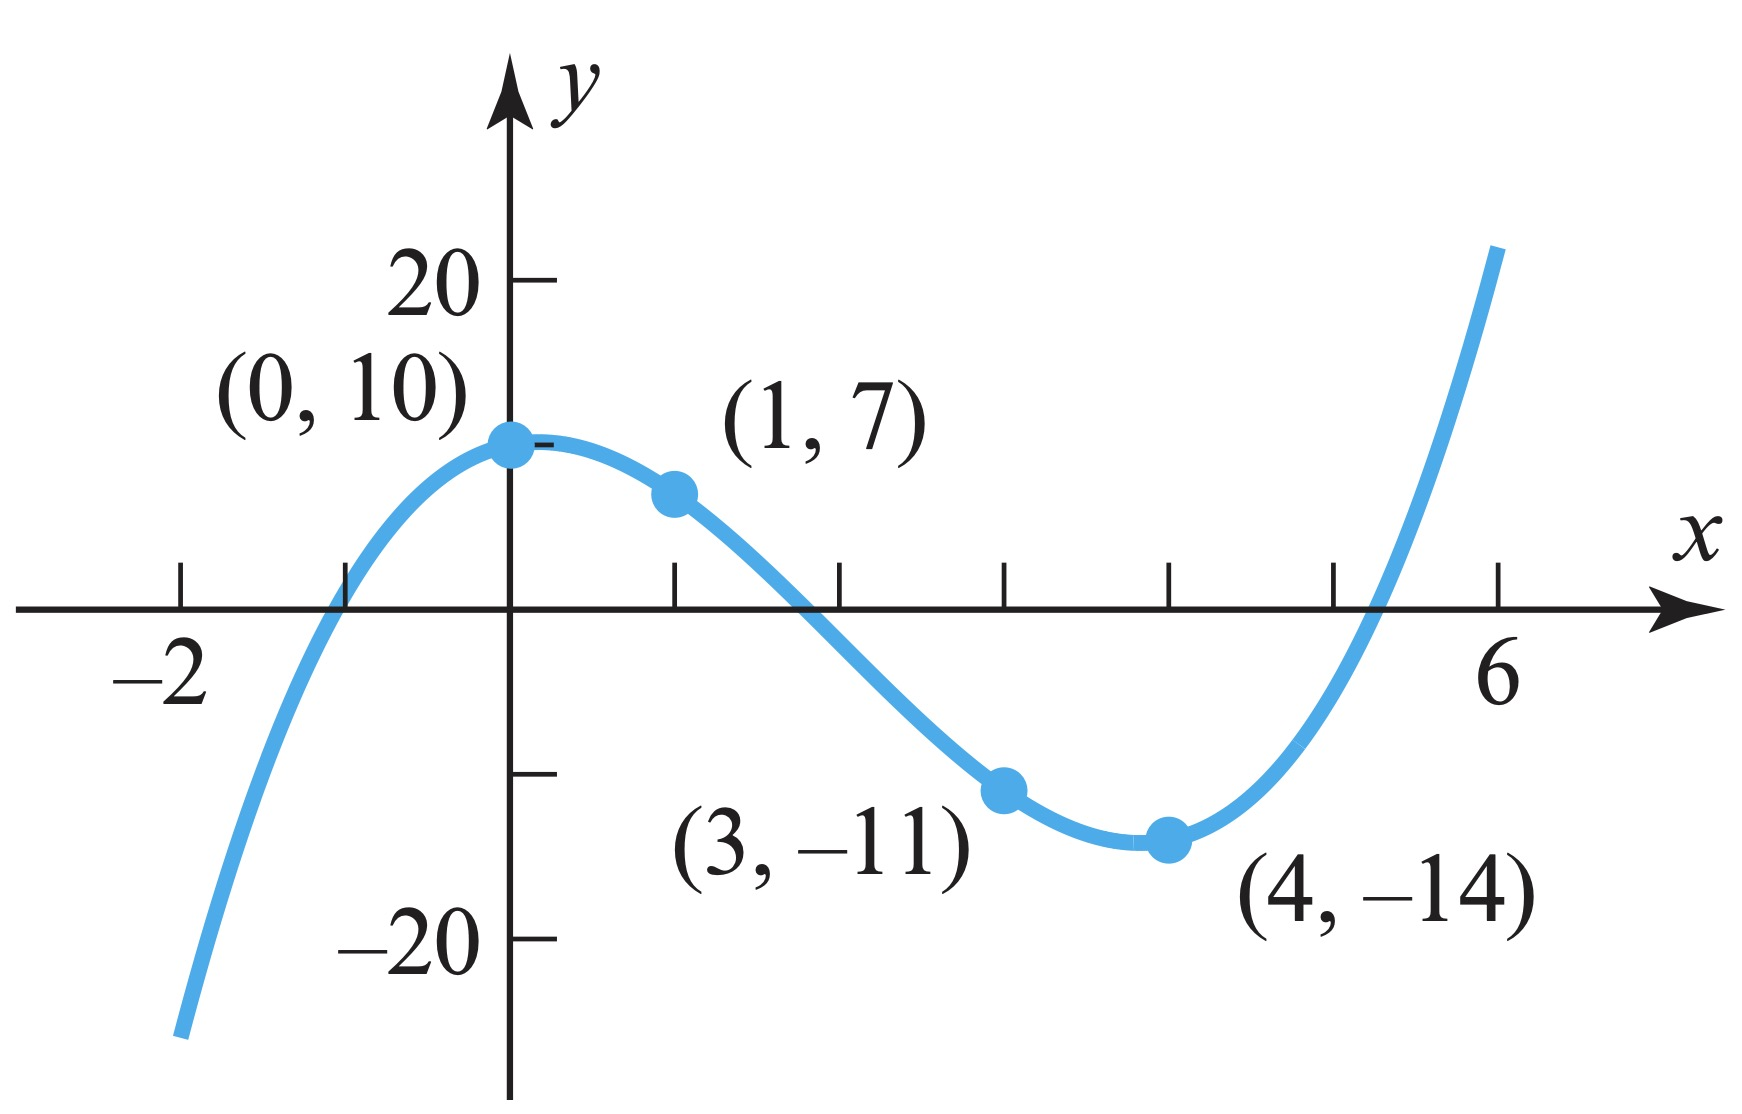
\includegraphics[width=0.4\textwidth]{figures/Curve.JPG}
\end{figure}
\hrline

\cyanbox{Solution:}
$$y=ax^3+bx^2+cx+d \tab \seteqno{1}$$

If the poly $(1)$ passes through the points $(0,10)$, $(1,7)$, $(3,-11)$, $(4,-14)$ then,
\begin{align*}
   d &= 10 \\
   a+b+c+d&=7 \\
   27a + 9b + 3c + d &= -11 \\
   64a + 16b + 4c + d &= -14
\end{align*}
\vspace{-1.5\baselineskip}

\begin{equation*}
   \left.\begin{array}{rl}
   a+b+c&=-3 \\
   27a+9b+3c &= -21 \\
   64a+16b+4c &= -24
   \end{array}\right\} \tab \seteqno{1}
\end{equation*}

In matrix form $A \mathbf{x}=\mathbf{b}$,
\begin{equation*}
   A=\begin{fmatrix}{lll}
   1 & 1 & 1 \\ 27 & 9 & 3 \\ 64 & 16 & 4
   \end{fmatrix}, \quad
   \mathbf{x} \ = \ \begin{fmatrix}{l}
   a \\ b \\ c
   \end{fmatrix}, \quad
   \mathbf{b} \ = \ \begin{fmatrix}{r}
   -3 \\ -21 \\ -24
   \end{fmatrix}
\end{equation*}

\begin{equation*}
\begin{aligned}
   &(A \mid \mathbf{b}) \ = \ \begin{fmatrix}{lll|l}
      1 & 1 & 1 & -3 \\ 27 & 9 & 3 & -21 \\ 64 & 16 & 4 & -24
   \end{fmatrix}
   \ro[R3'=\frac{R3}{4}]{R2'=\frac{R2}{3}}
   \begin{fmatrix}{lll|l}
      1 & 1 & 1 & -3 \\ 9 & 3 & 1 & -7 \\ 16 & 4 & 1 & -6
   \end{fmatrix}\\\\
   &\ro[R3'=R3-16R1]{R2'=R2-9R1}
   \begin{fmatrix}{lll|l}
      1 & 1 & 1 & -3 \\ 0 & -6 & -8 & 20 \\ 0 & -12 & -15 & 42
   \end{fmatrix}
   \ro{R3'=R3-2R2}
   \begin{fmatrix}{lll|l}
      1 & 1 & 1 & -3 \\ 0 & -6 & -8 & 20 \\ 0 & 0 & 1 & 2
   \end{fmatrix}
\end{aligned}
\end{equation*}

The corresponding linear system,
\begin{equation*}
   \begin{array}{rl}
      a+b+c&=-3 \\ -6b-8c &= 20 \\ c &= 2
   \end{array}
\end{equation*}

By backward substitution,
\begin{equation*}
   \begin{array}{rl}
      c&=2 \\ b &=-6 \\ a &= 1
   \end{array}
\end{equation*}

$\therefore$ The required poly is \tab \scalebox{1.15}{$y=x^3-6x^2+2x+10$}


\pagebreak

\vspace{10ex}
\cyanbox{Problem:} Find the coefficients \scalebox{1.15}{$a$}, \scalebox{1.15}{$b$}, \scalebox{1.15}{$c$}, and \scalebox{1.15}{$d$} so that the circle shown in the accompanying figure is given by the equation
\scalebox{1.15}{$ax^2+ay^2+bx+cy+d=0$}.

\begin{figure}[h]
   \centering
   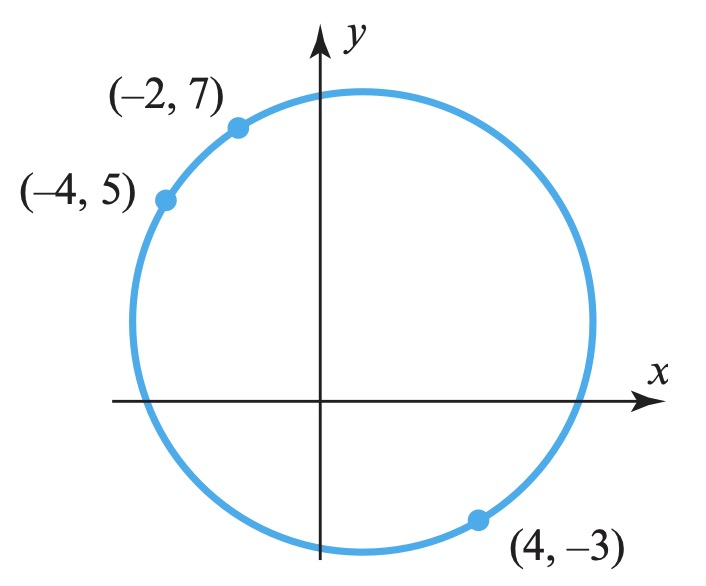
\includegraphics[width=0.4\textwidth]{figures/Circle.JPG}
\end{figure}
\hrline
\cyanbox{Solution:}
$$ax^2+ay^2+bx+cy+d=0 \tab \seteqno{1}$$

If the poly $(1)$ passes through the points $(-4,5)$, $(-2,7)$, $(4,3)$ then,

\begin{equation*}
   \begin{array}{rl}
      16a+25a-4b+5c+d & =0 \\
      4a+49a-2b+7c+d & =0 \\
      16a+9a+4b-3c+d & =0
   \end{array}
   \tabs \Rightarrow \tabs
   \begin{array}{rl}
      41a-4b+5c+d & =0 \\
      53a-2b+7c+d & =0 \\
      25a+4b-3c+d & =0
   \end{array}
\end{equation*}
\begin{equation*}
\left.\begin{array}{rl}
   d+5c-4b+41a & =0 \\
   d+7c-2b+53a & =0 \\
   d-3c+4b+25a & =0
\end{array}\right\} \tab \seteqno{1}
\end{equation*}

In matrix form $A \mathbf{x}=\mathbf{b}$,
\begin{equation*}
   A=\begin{fmatrix}{cccc}
   1 & 5 & -4 & 41 \\ 1 & 7 & -2 & 53 \\ 1 & -3 & 4 & 25
   \end{fmatrix}, \quad
   \mathbf{x} \ = \ \begin{fmatrix}{l}
   d \\ c \\ b \\ a
   \end{fmatrix}, \quad
   \mathbf{b} \ = \ \begin{fmatrix}{r}
   0 \\ 0 \\ 0
   \end{fmatrix}
\end{equation*}

\begin{equation*}
\begin{aligned}
  &(A \mid \mathbf{b}) \ = \ \begin{fmatrix}{cccc|c}
   1 & 5 & -4 & 41 & 0 \\
   1 & 7 & -2 & 53 & 0 \\
   1 & -3 & 4 & 25 & 0
   \end{fmatrix}
   \ro[R3'=R3-R1]{R2'=R2-R1}
   \begin{fmatrix}{cccc|c}
      1 & 5 & -4 & 41 & 0 \\
      0 & 2 & 2 & 12 & 0 \\
      0 & -8 & 8 & -16 & 0
   \end{fmatrix}\\\\
   &\ro{R3'=R3+4R2}
   \begin{fmatrix}{cccc|c}
      1 & 5 & -4 & 41 & 0 \\
      0 & 2 & 2 & 12 & 0 \\
      0 & 0 & 16 & 32 & 0
   \end{fmatrix}
   \ro[R2'=\frac{R2}{2}]{R3'=\frac{R3}{16}}
   \begin{fmatrix}{cccc|c}
      1 & 5 & -4 & 41 & 0 \\
      0 & 1 & 1 & 6 & 0 \\
      0 & 0 & 1 & 2 & 0
   \end{fmatrix}
\end{aligned}
\end{equation*}


\vspace{3ex}
The corresponding linear system,
\vspace{-0.75\baselineskip}
\begin{align*}
   d+5c-4b+41a &=0 \\
   c+b+6a &=0 \\
   b+2a &=0
\end{align*}

Let \ \scalebox{1.2}{$a=r$}, \tab therefore \ \ \scalebox{1.2}{$b=-2r; \tab c=-4r; \tab d=-29r$}

\vspace{2ex}
Substituting this values in equation $(1)$,
\vspace{-0.75\baselineskip}
\begin{align*}
   & = r(x^2+y^2-2x-4y-29)\\
   & = x^2+y^2-2x-4y-29 \tabs \tabs [\text{where } r=1]
\end{align*}

\vspace{-0.75\baselineskip}
$\therefore$ The required poly is \tab $x^2+y^2-2x-4y-29$

\end{document}
